\documentclass[conference]{IEEEtran}
\IEEEoverridecommandlockouts
\usepackage{cite}
\usepackage{amsmath,amssymb,amsfonts}
\usepackage{algorithmic}
\usepackage{graphicx}
\usepackage{textcomp}
\usepackage{xcolor}
\usepackage{hyperref}
\usepackage{booktabs}
\usepackage{subcaption}
\graphicspath{{figures/}}
\def\BibTeX{{\rm B\kern-.05em{\sc i\kern-.025em b}\kern-.08em
    T\kern-.1667em\lower.7ex\hbox{E}\kern-.125emX}}
\begin{document}

\title{Extending Heterogeneity-Aware GPU Scheduling with Fragmentation Awareness\\
\thanks{*This paper was written as a final project report for Stanford's Advanced Networking and Distributed System CS244 course in Winter 2026.
Thanks to Dr. Keith Winstein and Dr. David Mazi\`eres for their guidance and review.}
}

\author{\IEEEauthorblockN{Varun Ramesh}
\IEEEauthorblockA{\textit{Stanford University} \\
\textit{Graduate Department of Engineering} \\
vramesh3@stanford.edu}
\and
\IEEEauthorblockN{Jiayu Chang}
\IEEEauthorblockA{\textit{Stanford University} \\
\textit{Graduate Department of Engineering} \\
cjy1125@stanford.edu}
\and
\IEEEauthorblockN{Hyeonggyu Kim}
\IEEEauthorblockA{\textit{Stanford University} \\
\textit{Graduate Department of Engineering} \\
hgk@stanford.edu}
\and
\hspace*{6.5cm}\IEEEauthorblockN{Stefan Gabriel Ene}
\IEEEauthorblockA{\hspace*{6.5cm}\textit{Stanford University} \\
\hspace*{6.5cm}\textit{Graduate Department of Engineering} \\
\hspace*{6.5cm}enegstef@stanford.edu}
}

\maketitle

\begin{abstract}
We integrate Fragmentation Gradient Descent (FGD) into Gavel's heterogeneity-aware scheduling framework through a two-stage design: Gavel's policy layer determines GPU type and quantity allocations via linear programming, while FGD selects the specific nodes that minimize fragmentation growth.
We replicate both systems independently -- validating Gavel on the Microsoft Philly trace (504 experiments) and FGD on the Alibaba GPU-sharing trace (6 placement policies across 1,200 nodes) -- then evaluate the combined scheduler on two Alibaba cluster topologies under both Max-Min Fairness and FIFO policies (900 total experiments).
Our results reveal that fragmentation-aware placement reduces the fragmentation rate by 30--40\% on clusters with mixed node sizes (1--8 GPUs per node), but provides no benefit on uniform-node clusters where all placement strategies converge.
This finding demonstrates that the value of fragmentation-aware scheduling depends on \textit{node topology diversity}, not GPU type heterogeneity, and that effective cluster scheduling requires jointly considering allocation policy, placement strategy, and physical topology.
\end{abstract}

\begin{IEEEkeywords}
GPU sharing, fragmentation, heterogeneity-aware, scheduling policies, workload traces, distributed training
\end{IEEEkeywords}


\section{Introduction}
GPU cluster scheduling for deep learning has evolved as organizations deploy increasingly diverse hardware for training and inference workloads.
In production environments, GPU utilization averages between 25\% and 50\% \cite{FGD}, motivating the adoption of GPU sharing where multiple tasks run on a single physical GPU through partial resource allocation.

While GPU sharing improves aggregate utilization, it introduces \textit{resource fragmentation}: remaining capacity on individual devices may be too small to satisfy subsequent requests, and these fragments cannot be consolidated across physical GPU boundaries.
Production trace analysis from Alibaba clusters shows that fragmentation renders 21\% to 42\% of unallocated GPU resources unusable during normal operation \cite{ALIBABA, FGD}.

Separately, heterogeneous GPU clusters require scheduling policies that account for varying per-model speedups across accelerator types.
A ResNet-50 model sees 10x throughput improvement from K80 to V100, while A3C sees only 2x \cite{GAVEL}.

Two recent systems address complementary aspects of this problem.
Gavel \cite{GAVEL} expresses scheduling policies as optimization problems over an effective throughput abstraction, enabling heterogeneity-aware allocation with support for fairness, makespan minimization, and hierarchical policies -- but was validated exclusively on whole-GPU workloads where fragmentation does not arise.
FGD \cite{FGD} defines a statistical fragmentation measure and places tasks toward the steepest descent of this measure, reducing unallocated GPUs by up to 49\% -- but operates under FIFO ordering without a flexible policy framework.

\subsection{Contribution}
We bridge these approaches through three contributions:
\begin{enumerate}
\item Independent replication of both Gavel and FGD, validating against published results on their respective traces.
\item Integration of FGD placement into Gavel's two-stage architecture, preserving policy-level optimization while adding fragmentation awareness.
\item A comparative evaluation revealing that fragmentation reduction depends on \textit{node topology diversity} (mixed node sizes), not GPU type heterogeneity -- a finding neither original paper addresses.
\end{enumerate}

\section{Background \& Related Work}

\subsection{Heterogeneity-Aware Scheduling with Gavel}
Modern GPU clusters contain multiple accelerator generations with widely varying per-model throughputs.
Gavel \cite{GAVEL} addresses this by expressing scheduling policies as optimization problems over allocation matrices, where each entry specifies the fraction of wall-clock time a job spends on a given accelerator type.

As illustrated in Fig.~\ref{fig:gavel_algorithm}, Gavel profiles each job's throughput on every GPU type, then solves a Max-Min Fairness LP to maximize the minimum effective throughput across all jobs, subject to per-type capacity constraints.
The result assigns each job to the GPU types where it runs fastest, while maintaining fair sharing across the cluster.
A round-based mechanism maps these fractional allocations to physical resource assignments using priority scores.

\begin{figure}[t]
  \centering
  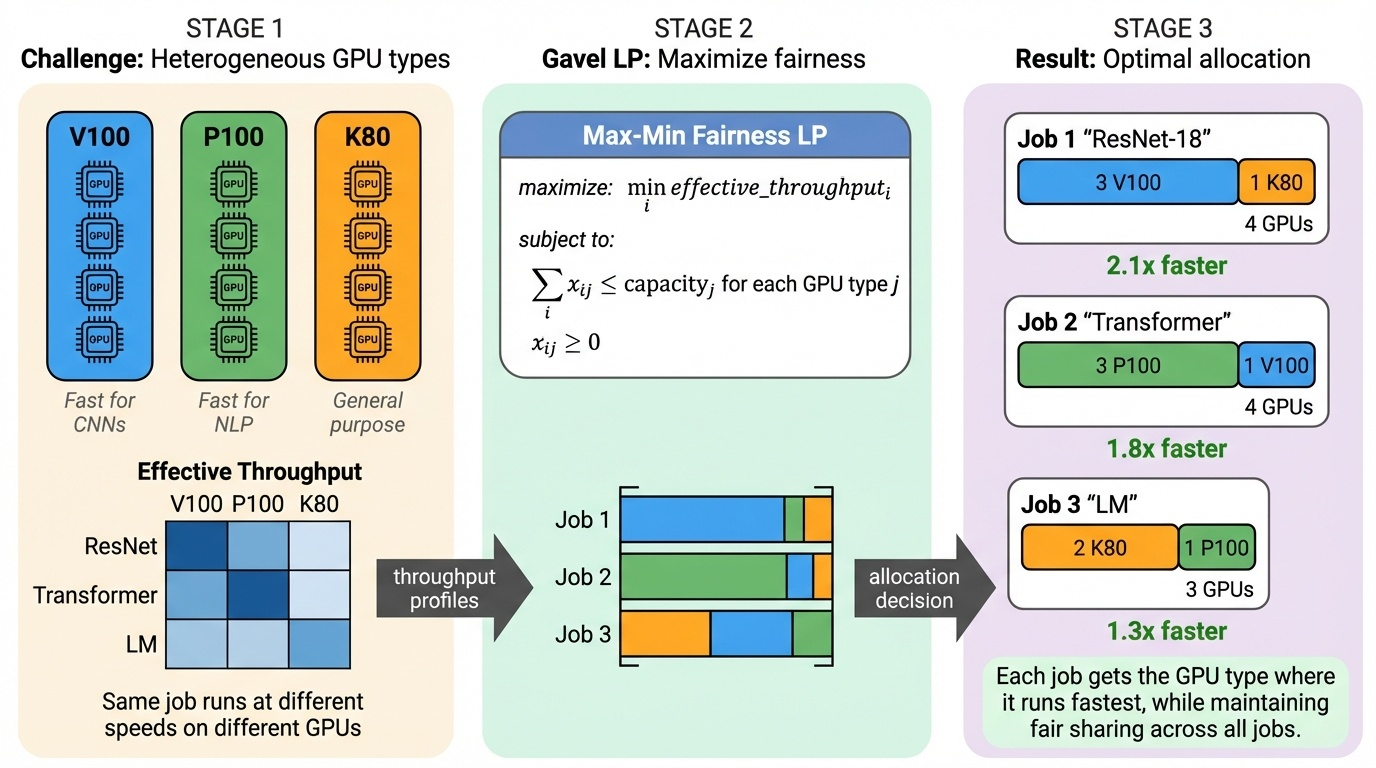
\includegraphics[width=\columnwidth]{fig2_gavel_algorithm.png}
  \caption{Gavel's heterogeneity-aware allocation. Stage 1: Each job exhibits different throughputs across GPU types (e.g., ResNet runs fastest on V100, Transformer on P100). Stage 2: The Max-Min Fairness LP allocates time fractions per GPU type to maximize the minimum effective throughput. Stage 3: Each job receives GPUs on its best types -- ResNet-18 gets 1.3--2.1x speedup over a heterogeneity-agnostic baseline.}
  \label{fig:gavel_algorithm}
\end{figure}

Gavel generalizes policies including Least Attained Service (max-min fairness), finish-time fairness, FIFO, and makespan minimization.
However, Gavel was validated exclusively on the Microsoft Philly trace, which contains only whole-GPU job requests, and its placement logic does not consider fragmentation from partial GPU allocations.

\subsection{Fragmentation-Aware Placement with FGD}
GPU sharing introduces \textit{resource fragmentation}: remaining capacity on individual devices may be too small to satisfy subsequent requests, and unlike memory or disk fragmentation, GPU fragments cannot be consolidated across physical device boundaries.
In Alibaba's production deployment, tasks receive partial GPU allocations at a granularity of 0.01 GPUs \cite{FGD}.

FGD \cite{FGD} addresses this through a statistical fragmentation measure that computes, for each node, the expected number of GPUs that cannot serve a randomly sampled task from the workload.
This captures both \textit{deficient} fragmentation (insufficient GPU capacity) and \textit{stranded} fragmentation (sufficient GPU but insufficient co-located CPU or memory).
As illustrated in Fig.~\ref{fig:fgd_algorithm}, FGD evaluates every eligible node for each incoming task, computes the fragmentation increment at each, and selects the node with the minimum gradient.

\begin{figure}[t]
  \centering
  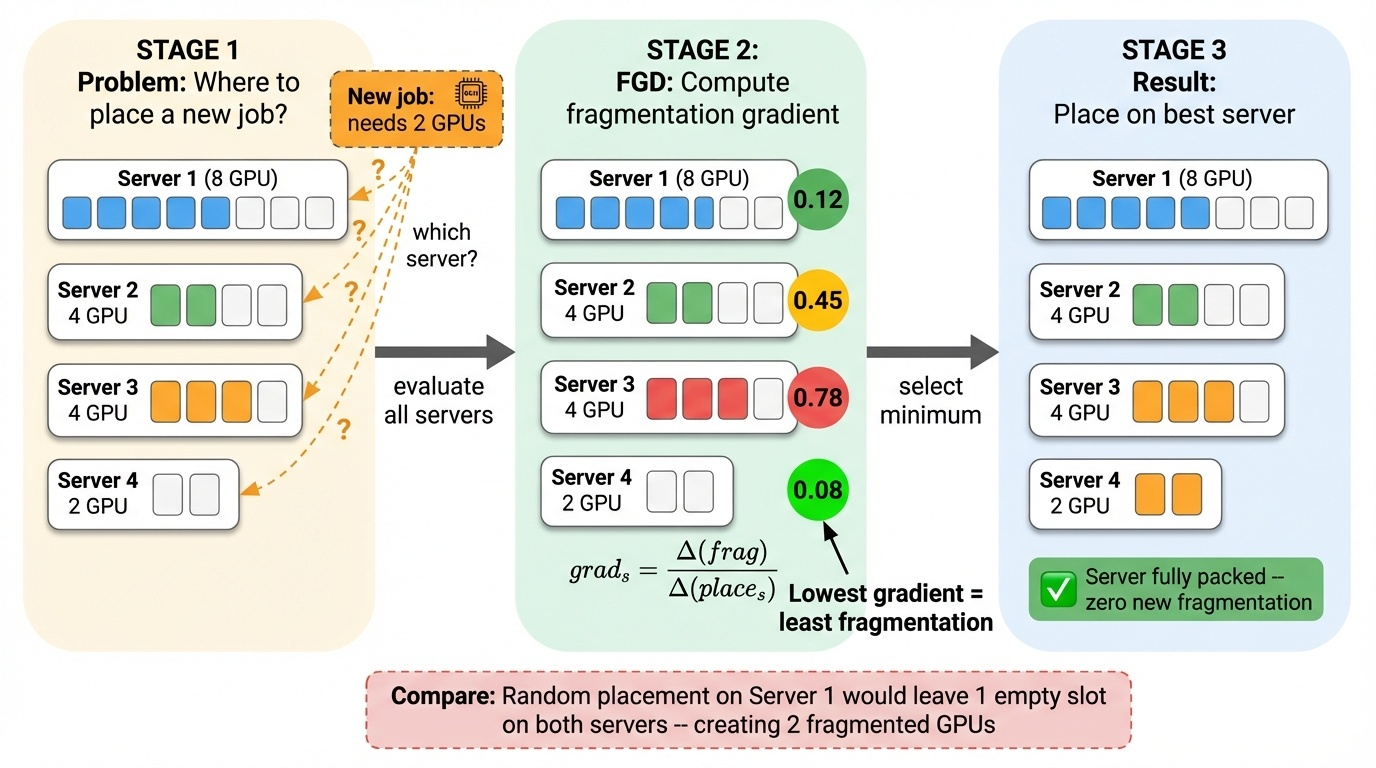
\includegraphics[width=\columnwidth]{fig3_fgd_algorithm.png}
  \caption{FGD placement algorithm. For a 2-GPU job, FGD computes the fragmentation gradient at each server. Server 4 (gradient = 0.08) is selected because placing the job there fully packs the server, creating zero new fragmentation. Random placement on Server 1 would scatter fragments across two servers.}
  \label{fig:fgd_algorithm}
\end{figure}

\subsection{Other Related Work}
Relevant GPU work in this area appears throughout past literature.
Salus \cite{SALUS} provides fine-grained GPU sharing primitives that enable memory-safe co-location of multiple DNN training jobs on a single GPU through fast job switching and memory sharing.
Gandiva \cite{GANDIVA} introduces time-slicing and migration mechanisms for GPU clusters, exploiting intra-job predictability to improve utilization.
Tiresias \cite{TIRESIAS} schedules distributed DNN training jobs using Least Attained Service with a two-dimensional framework that considers both GPU allocation and placement.


\section{Methodology}

Our approach proceeds in three phases: independent replication of each baseline, integration into a combined system, and comparative evaluation.
A key challenge is that Gavel and FGD use fundamentally different evaluation methodologies, illustrated in Fig.~\ref{fig:eval_methodology}.

\begin{figure}[t]
  \centering
  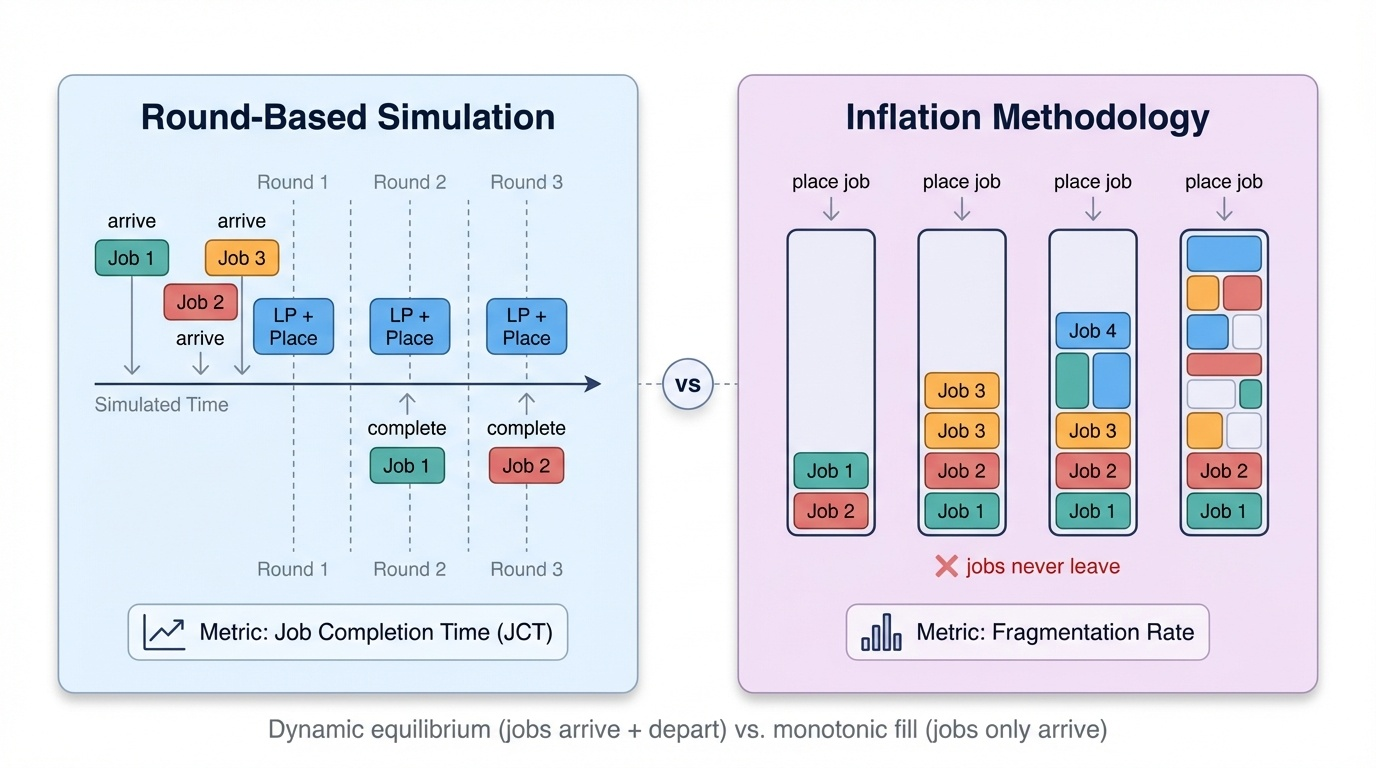
\includegraphics[width=\columnwidth]{fig4_eval_methodology.png}
  \caption{Evaluation methodology comparison. Left: Gavel's round-based simulation models dynamic job arrivals and departures in a steady-state equilibrium, measuring job completion time (JCT). Right: FGD's inflation methodology monotonically fills the cluster (jobs arrive but never depart), measuring fragmentation rate as utilization increases. Our combined evaluation bridges both approaches.}
  \label{fig:eval_methodology}
\end{figure}

\subsection{Phase 1: Baseline Replication}
We replicate Gavel's scheduling simulator using round-based simulation and validate against published results on the Microsoft Philly trace (108 GPUs: 36 V100, 36 P100, 36 K80).
In parallel, we replicate FGD's scheduler using the inflation methodology and validate against published results on the Alibaba v2023 trace \cite{ALIBABA} (Cluster H: 5,592 GPUs across 1,200 nodes with mixed node sizes of 1, 2, 4, and 8 GPUs).

\subsection{Phase 2: Integration}
We integrate FGD's placement into Gavel's scheduling framework as a two-stage architecture (Fig.~\ref{fig:architecture}).
Gavel's policy layer first solves a linear program to determine target time-fraction allocations per GPU type.
FGD then operates at the placement level: once Gavel determines which job runs in a given round and on which accelerator type, FGD computes the fragmentation gradient at each candidate node within that type and selects the node with the minimum increment.
This preserves Gavel's policy-level optimization while adding fragmentation awareness at the physical resource layer.

\subsection{Phase 3: Evaluation}
We evaluate three configurations: Gavel alone, standalone FGD, and combined Gavel+FGD.
For the combined evaluation, we test on two Alibaba cluster topologies to isolate the effect of node structure on fragmentation:

\begin{table}[h]
\centering
\caption{Cluster configurations used in evaluation.}
\label{tab:clusters}
\begin{tabular}{lcc}
\toprule
\textbf{Property} & \textbf{Alibaba Split} & \textbf{Cluster H} \\
\midrule
Total GPUs & 6,212 & 5,592 \\
Nodes & 1,213 & 1,200 \\
GPU types & 12 (heterogeneous) & 1 (homogeneous) \\
GPUs/node & 8 (uniform) & 1, 2, 4, 8 (mixed) \\
Node sizes & All same per type & 462/310/228/200 \\
\bottomrule
\end{tabular}
\end{table}

Each combined configuration sweeps 15 arrival rates $\times$ 3 seeds under both Max-Min Fairness and FIFO allocation policies, with 4 placement strategies (Random, Strided, BestFit, FGD), totaling 720 experiments.

\begin{figure}[t]
  \centering
  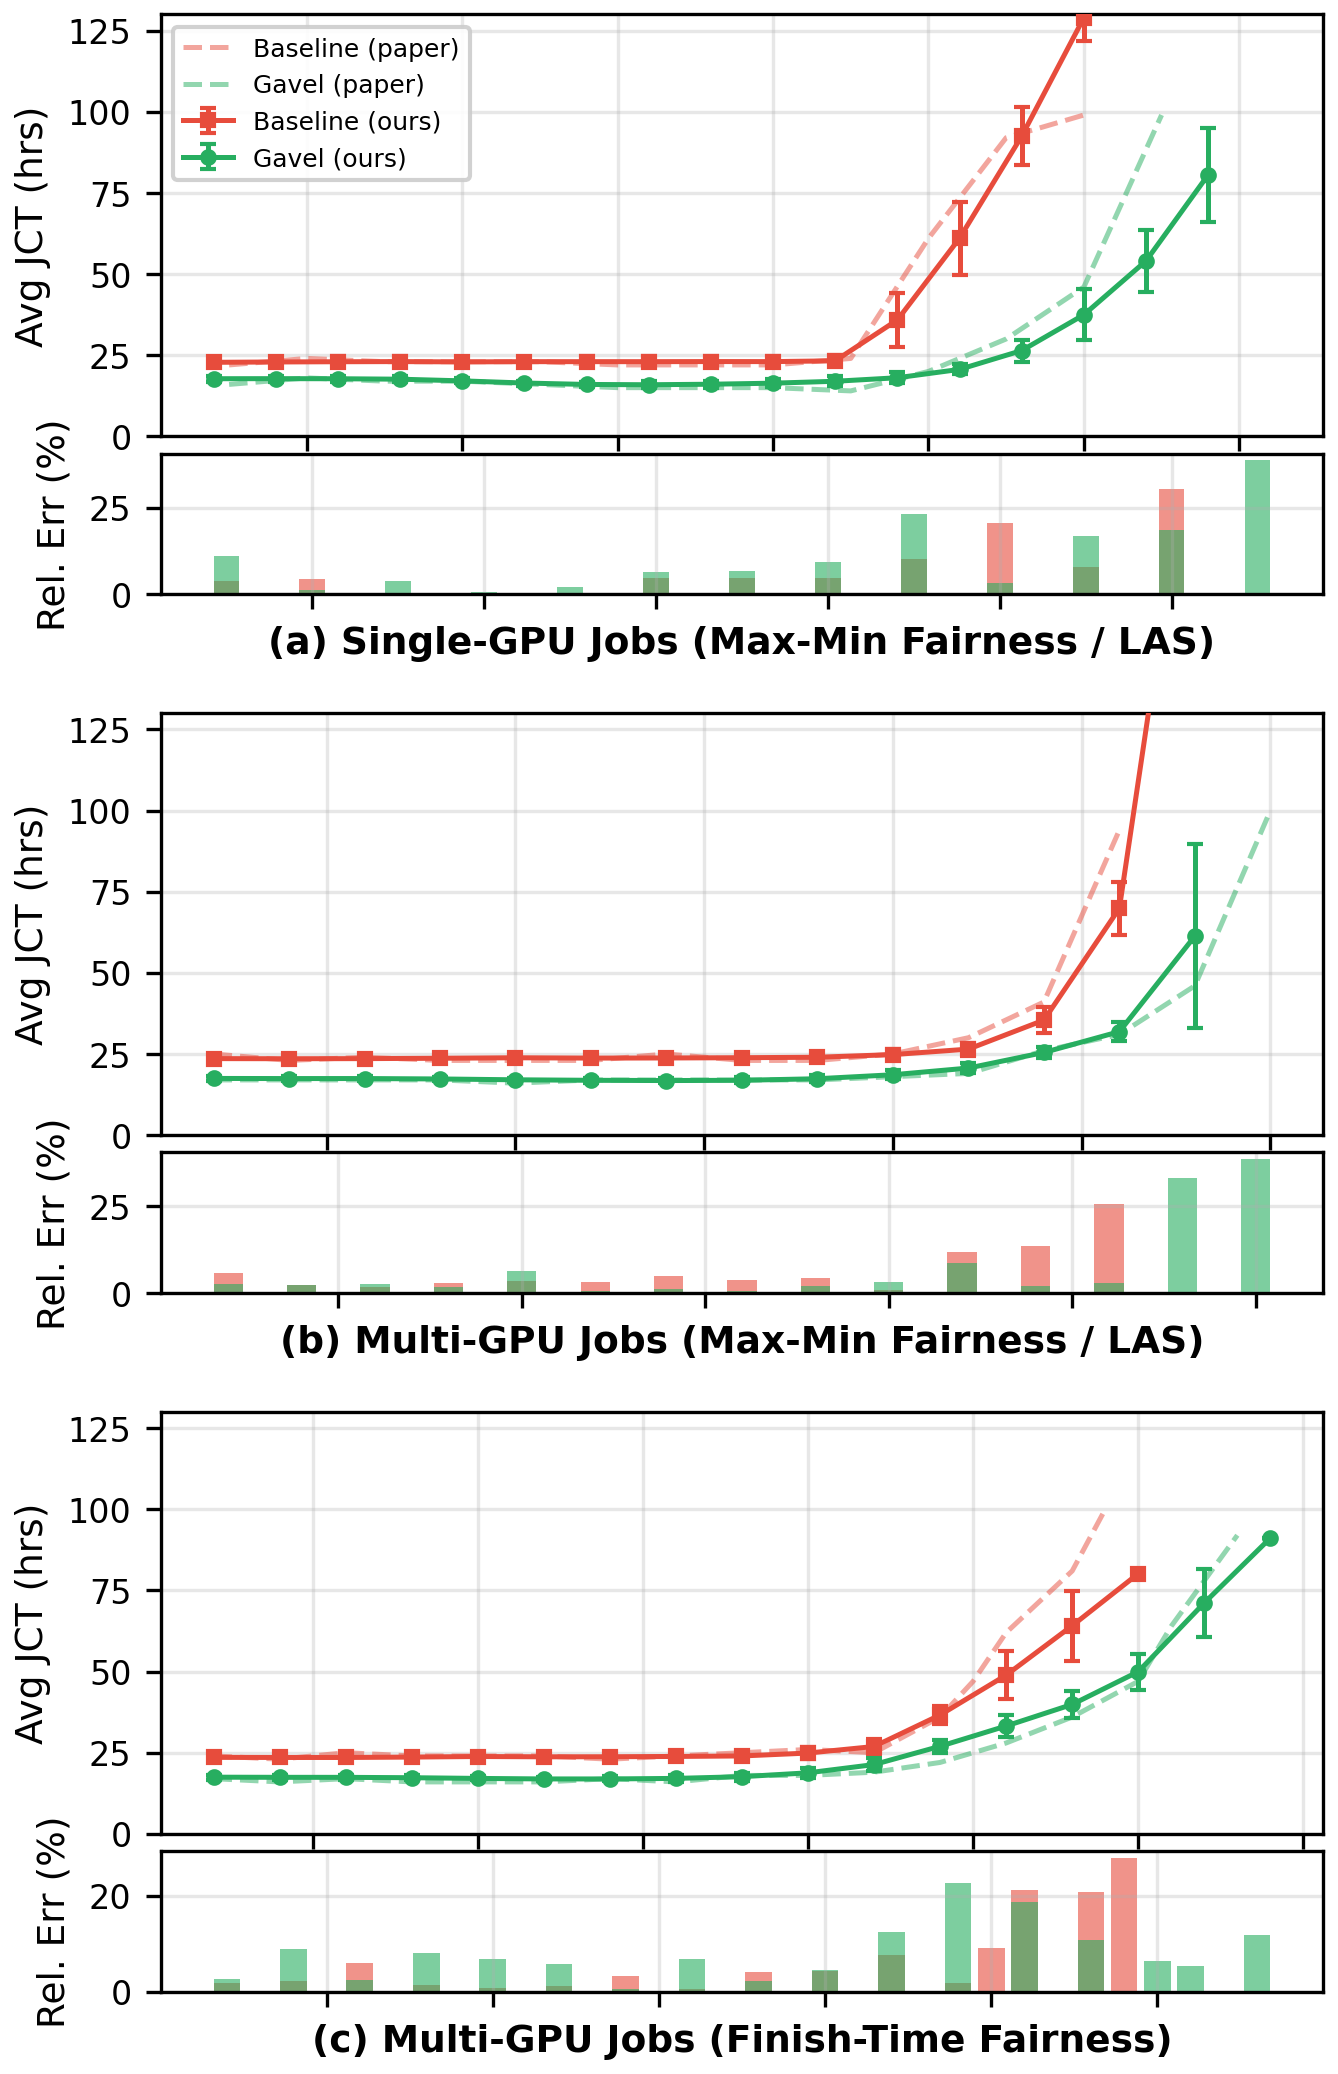
\includegraphics[width=\columnwidth]{fig_gavel_replication.png}
  \caption{Gavel replication results (Philly trace, 3 seeds). Solid: our results (mean $\pm$ std). Dashed: digitized paper reference. Relative error subplots below each panel. (a)~Single-GPU (MMF). (b)~Multi-GPU (MMF). (c)~Multi-GPU (Finish-Time Fairness). Error is small at sub-saturation loads and diverges near the saturation knee.}
  \label{fig:gavel_replication}
\end{figure}

\begin{figure}[t]
  \centering
  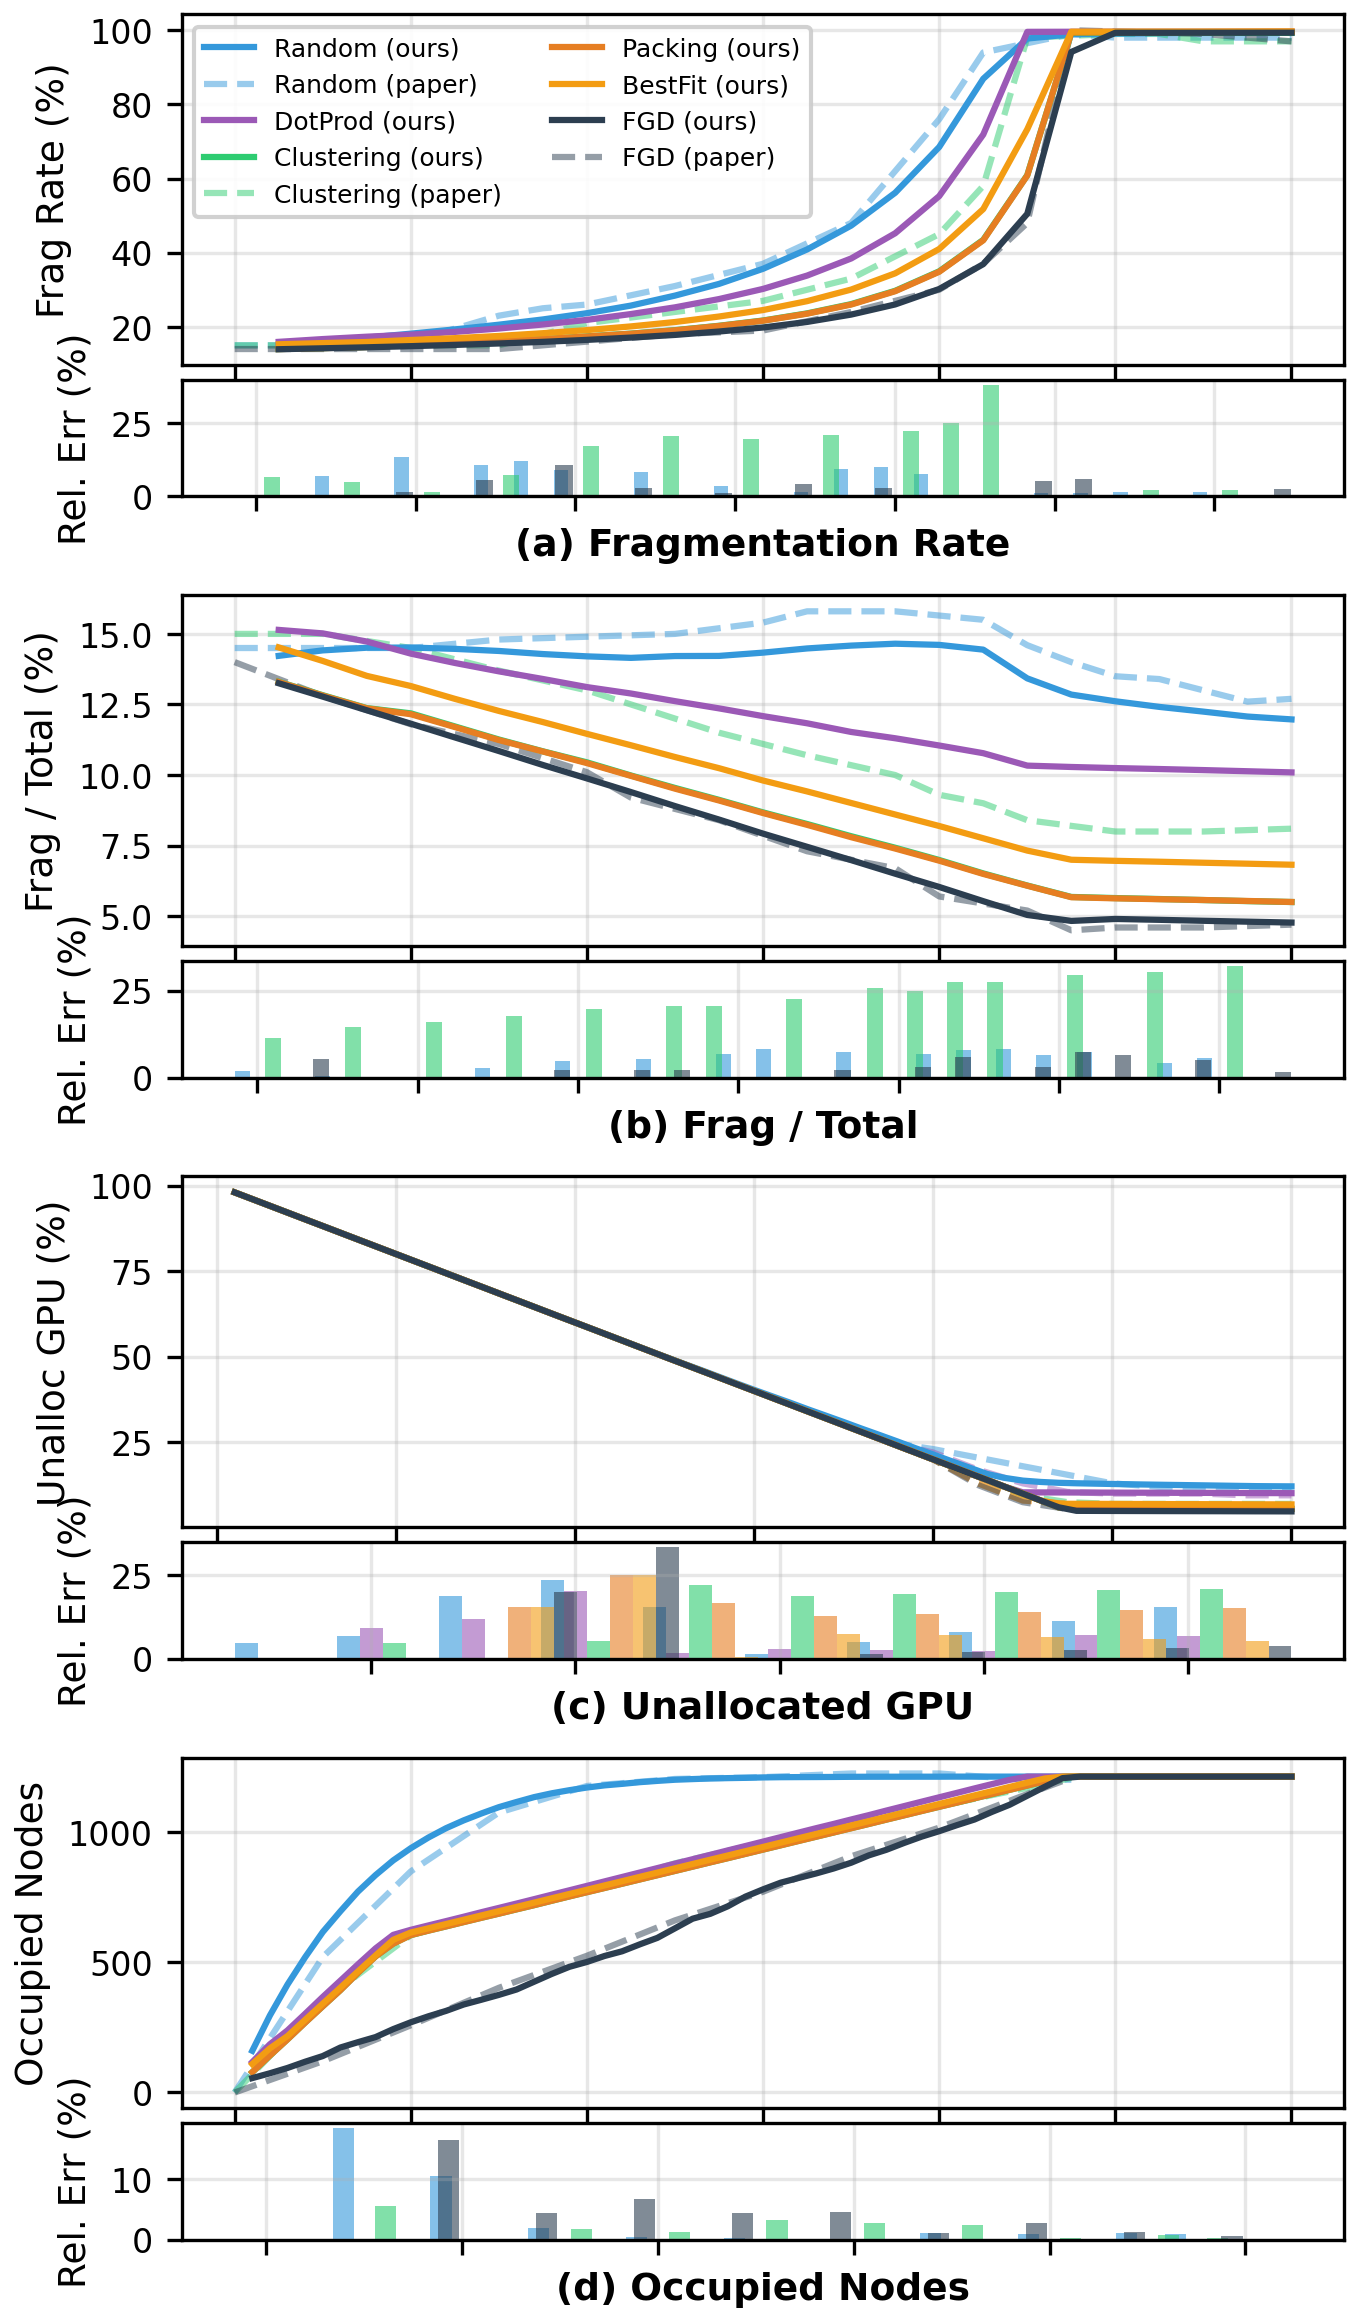
\includegraphics[width=\columnwidth]{fig_fgd_replication.png}
  \caption{FGD replication (Alibaba Cluster H, 6 policies, 10 runs). Solid: our results. Dashed: digitized paper reference. Relative error subplots below each panel. (a)~Fragmentation rate. (b)~Fragmented GPUs as \% of total. (c)~Unallocated GPU \%. (d)~Occupied nodes. FGD consistently achieves the lowest fragmentation and tightest packing.}
  \label{fig:fgd_replication}
\end{figure}

\begin{figure}[t]
  \centering
  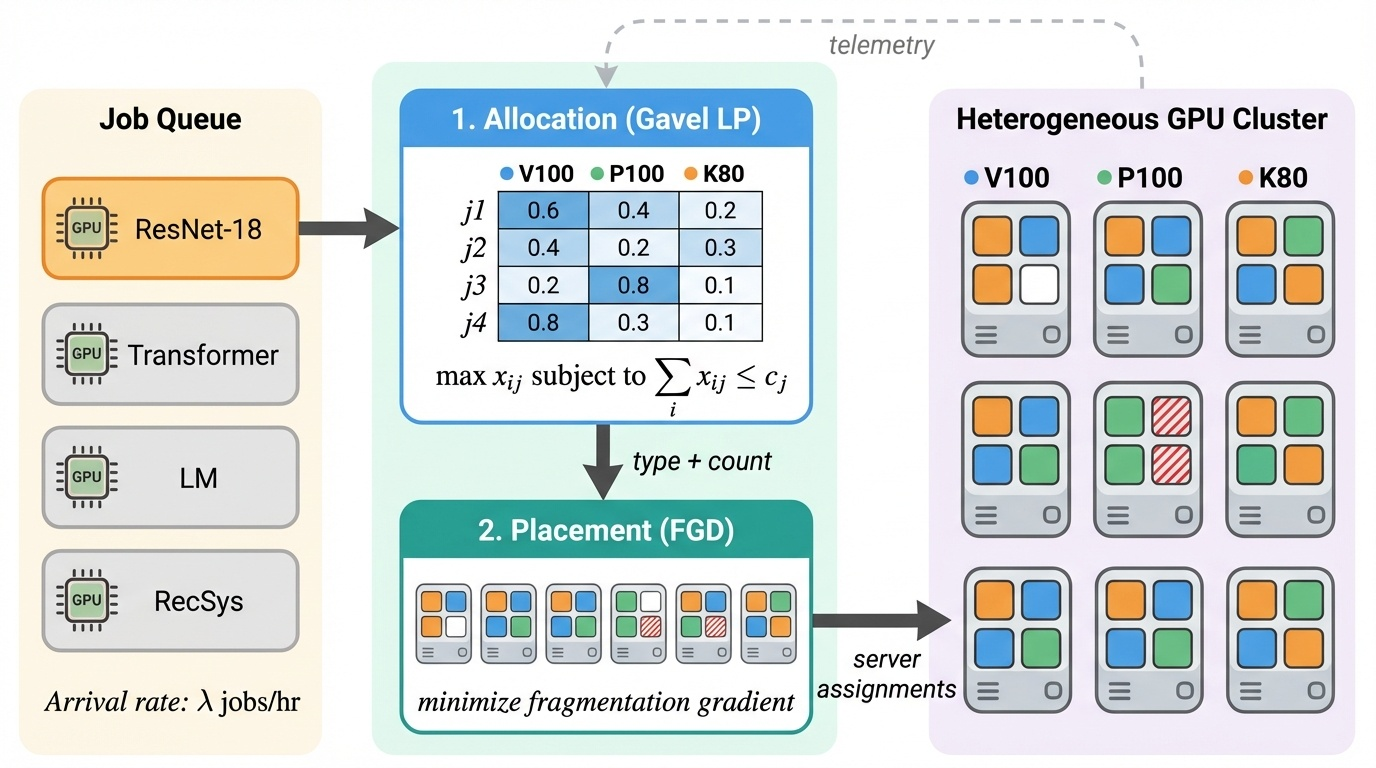
\includegraphics[width=\columnwidth]{fig1_architecture.png}
  \caption{Two-stage Gavel+FGD architecture. Stage 1 (Allocation): Gavel's LP computes time-fraction allocations across GPU types for each job. Stage 2 (Placement): FGD evaluates the fragmentation gradient at each candidate node and selects the node that minimizes fragmentation growth. Telemetry from the cluster feeds back into both stages.}
  \label{fig:architecture}
\end{figure}

\section{Replication Results}

\subsection{Gavel Replication}
We ran 504 experiments across three figure configurations from the original Gavel paper \cite{GAVEL}: single-GPU jobs under Max-Min Fairness (Fig.~9 in original), multi-GPU jobs under Max-Min Fairness (Fig.~10), and multi-GPU jobs under Finish-Time Fairness (Fig.~11).
Each configuration sweeps job arrival rate from low load to saturation across 3 random seeds.

Fig.~\ref{fig:gavel_replication} overlays our replication (solid lines) against digitized reference curves from the original paper (dashed lines), with point-by-point absolute error shown in subplots below each panel.
Across all three configurations, Gavel's heterogeneity-aware policy reduces average JCT by 20--70\% compared to the heterogeneity-agnostic baseline.
At low-to-moderate load, the error subplots show close agreement (typically $<$5 hours deviation per point).
Larger deviations appear only in the saturation tail, where our simulator reports lower JCT at extreme arrival rates.

\subsubsection{Saturation Behavior at High Load}
The multi-GPU configurations (Fig.~\ref{fig:gavel_replication}, center and right panels) exhibit a sharp JCT inflection near 2.0--2.5 jobs/hr, where the cluster approaches saturation.
At this point, multi-GPU jobs consume enough resources that the scheduler can no longer maintain steady-state: incoming jobs accumulate in the queue faster than they complete, causing JCT to grow without bound.
Our replication saturates at a slightly higher arrival rate than the paper reference, producing the largest deviations (e.g., Fig.~10 Gavel at 3.0 jph: ours = 29.78 hrs vs. paper = 100 hrs).
This difference likely reflects implementation details in queue management and preemption handling that are underspecified in the original paper.
The sub-saturation error of 3.05 hours RMSE confirms that the core scheduling logic replicates accurately where the system operates in equilibrium.

\subsection{FGD Replication}
We replicate FGD's standalone evaluation on the Alibaba Cluster H using the inflation methodology from the original paper \cite{FGD}.
Six placement policies are compared: Random, DotProd, GpuClustering, GpuPacking, BestFit, and FGD.

Fig.~\ref{fig:fgd_replication} shows our replication of four key FGD metrics alongside digitized paper reference curves, with relative error subplots below each panel.
As cluster demand increases, all policies see rising fragmentation rates (Fig.~\ref{fig:fgd_replication}a), but FGD maintains the lowest rate throughout.
At 80\% demand, Random placement fragments 85\% of unallocated GPUs while FGD fragments only 42\%.
The fragmentation-to-total ratio (Fig.~\ref{fig:fgd_replication}b) shows FGD keeping fragmented resources below 8\% of total cluster capacity, with the tightest replication accuracy across all four metrics.
The relative error subplots confirm close agreement across the entire demand range, with the largest deviations in fragmentation rate at high demand where stochastic effects dominate.


\section{Combined Gavel+FGD Results}

We evaluate the integrated system (Fig.~\ref{fig:architecture}) on both Alibaba cluster topologies under four placement strategies: Random, Strided (Gavel's default sequential assignment), BestFit, and FGD.

\subsection{Cluster H (Mixed Node Sizes)}
Fig.~\ref{fig:combined_cluster_h} shows results on Cluster H, where nodes contain 1, 2, 4, or 8 GPUs.
FGD placement reduces fragmentation rate by 30--40\% relative to Random at moderate utilization (40--70\%).
BestFit achieves intermediate performance, while Strided (Gavel's default) performs comparably to Random.
This ordering -- FGD $<$ BestFit $<$ Random $\approx$ Strided -- holds under both Max-Min Fairness and FIFO, indicating that the placement benefit is \textit{independent of the allocation policy}.

The occupied nodes metric (bottom-right) reveals why: FGD consolidates jobs onto fewer nodes, keeping small nodes (1--2 GPU) empty and available for future jobs of matching size.
Random placement scatters jobs across all node sizes, creating fragments on nodes too small to absorb them.

\begin{figure}[t]
  \centering
  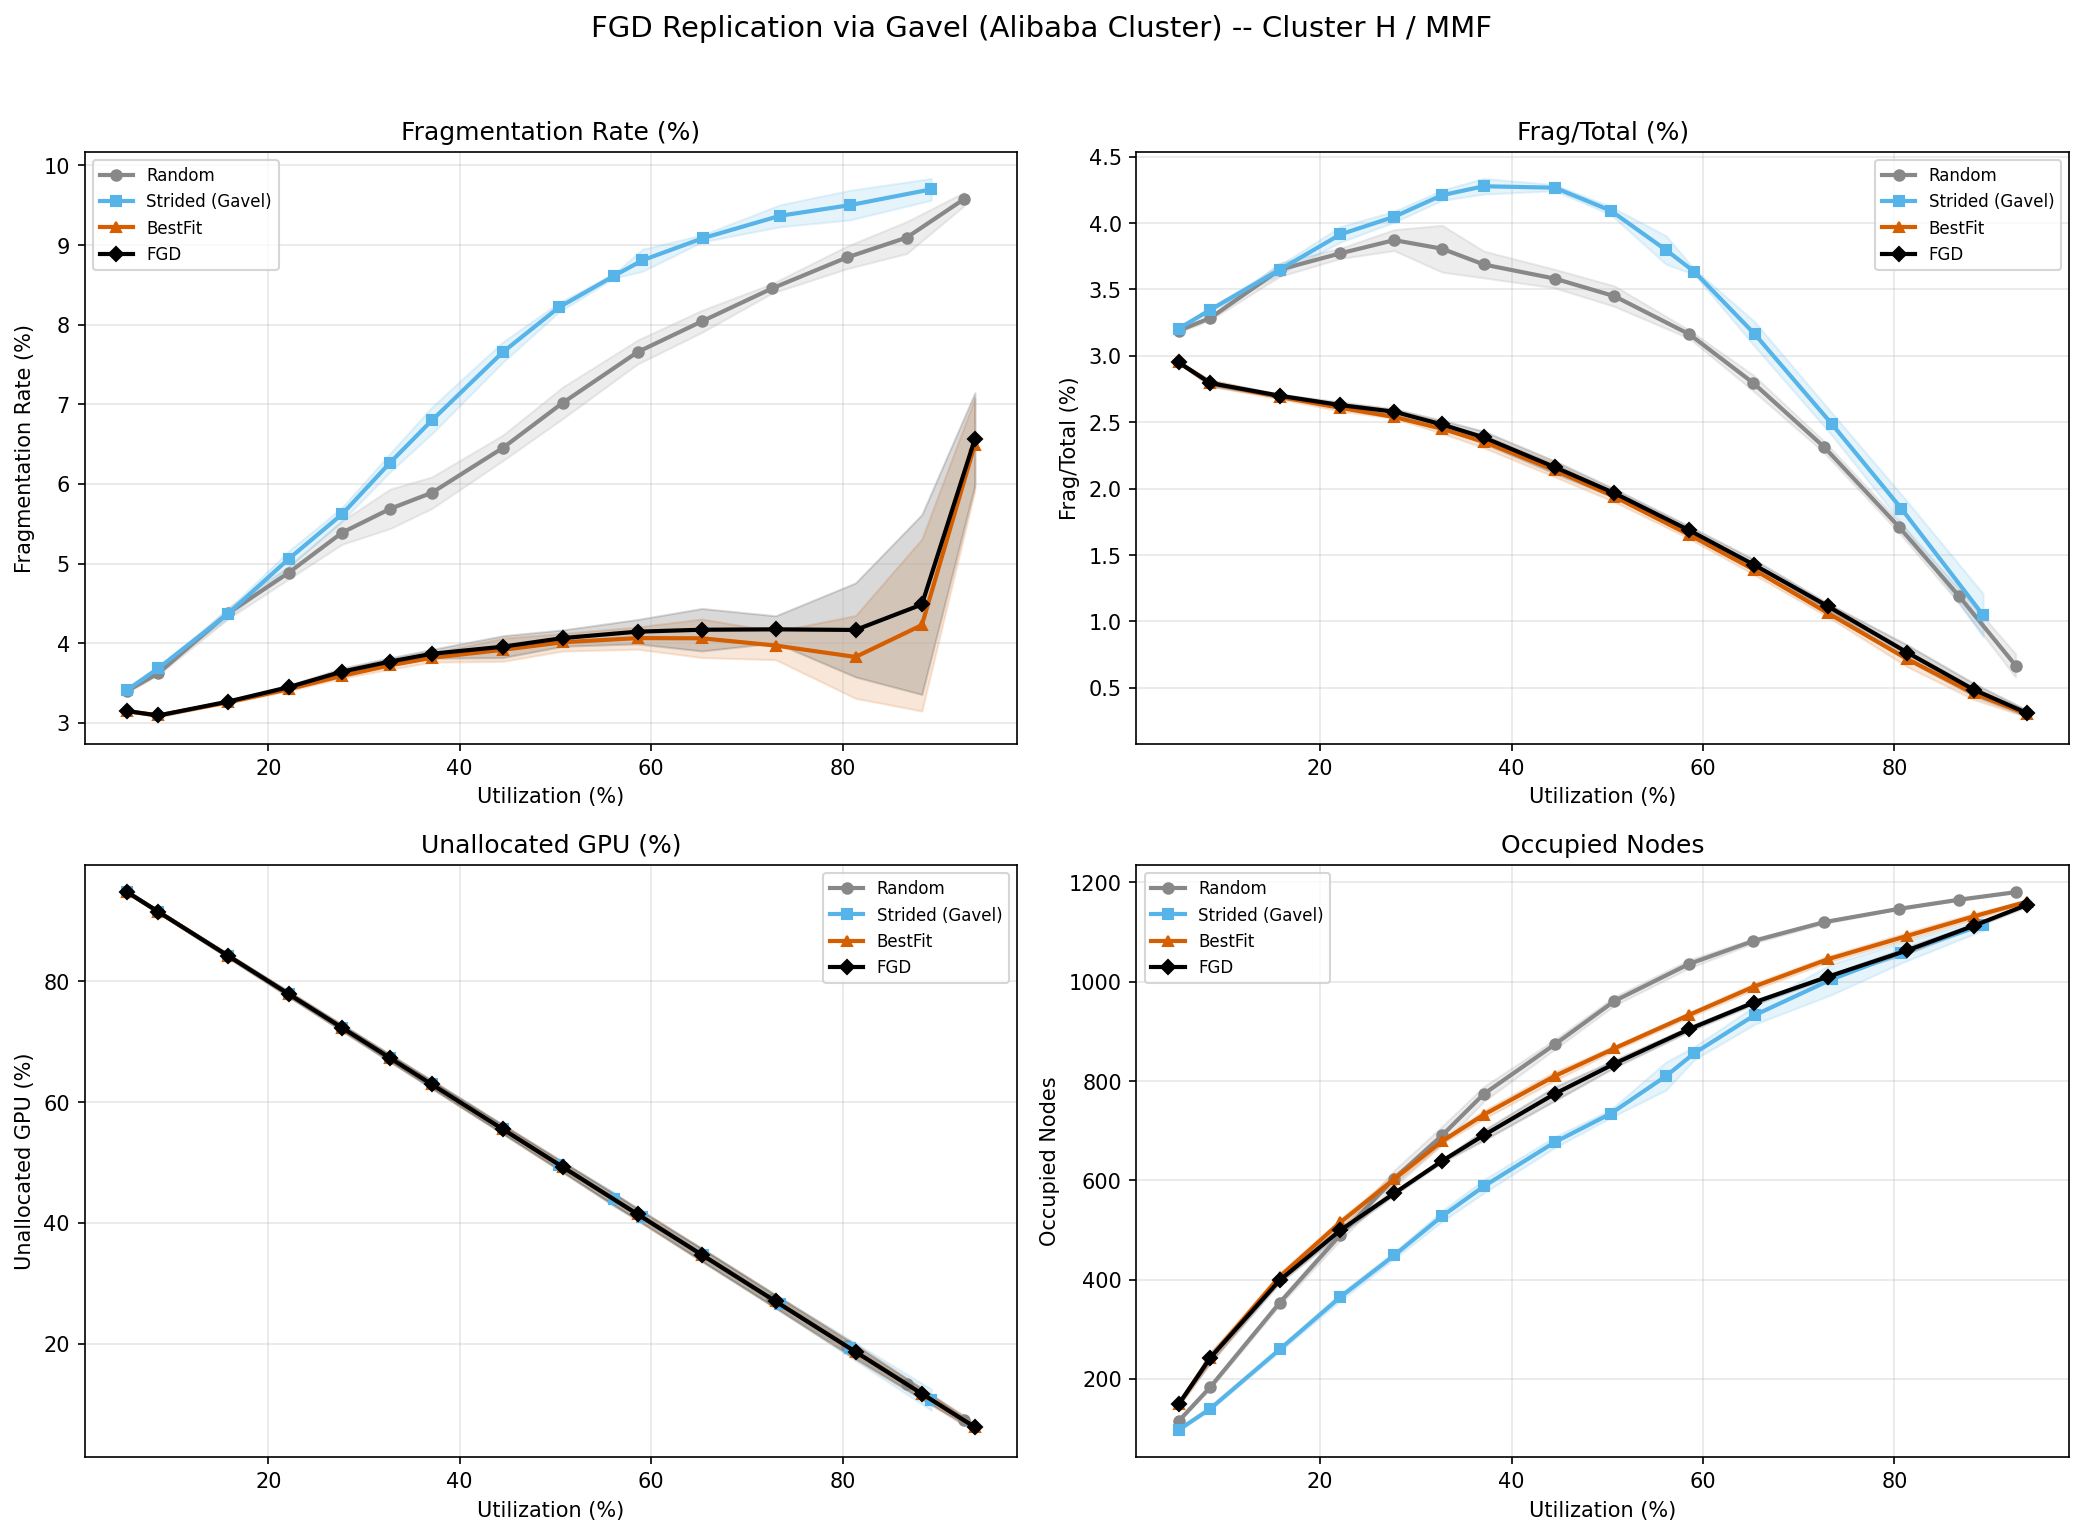
\includegraphics[width=\columnwidth]{fig7_combined_cluster_h.png}
  \caption{Gavel+FGD on Cluster H (mixed node sizes, Max-Min Fairness). FGD placement (black) reduces fragmentation rate by 30--40\% vs. Random (blue) at moderate utilization. BestFit (orange) is intermediate. Strided/Gavel default (brown) performs similarly to Random. Error bands: $\pm$1 std over 3 seeds.}
  \label{fig:combined_cluster_h}
\end{figure}

\subsection{Alibaba Split (Uniform Node Sizes)}
Fig.~\ref{fig:combined_uniform} shows results on the Alibaba Split cluster, where each GPU type has uniform 8-GPU nodes.
All four placement strategies produce nearly identical fragmentation rates across the entire utilization range.
When node sizes are uniform, placement strategy is irrelevant because any node of the correct type is equally suitable for any job.

\begin{figure}[t]
  \centering
  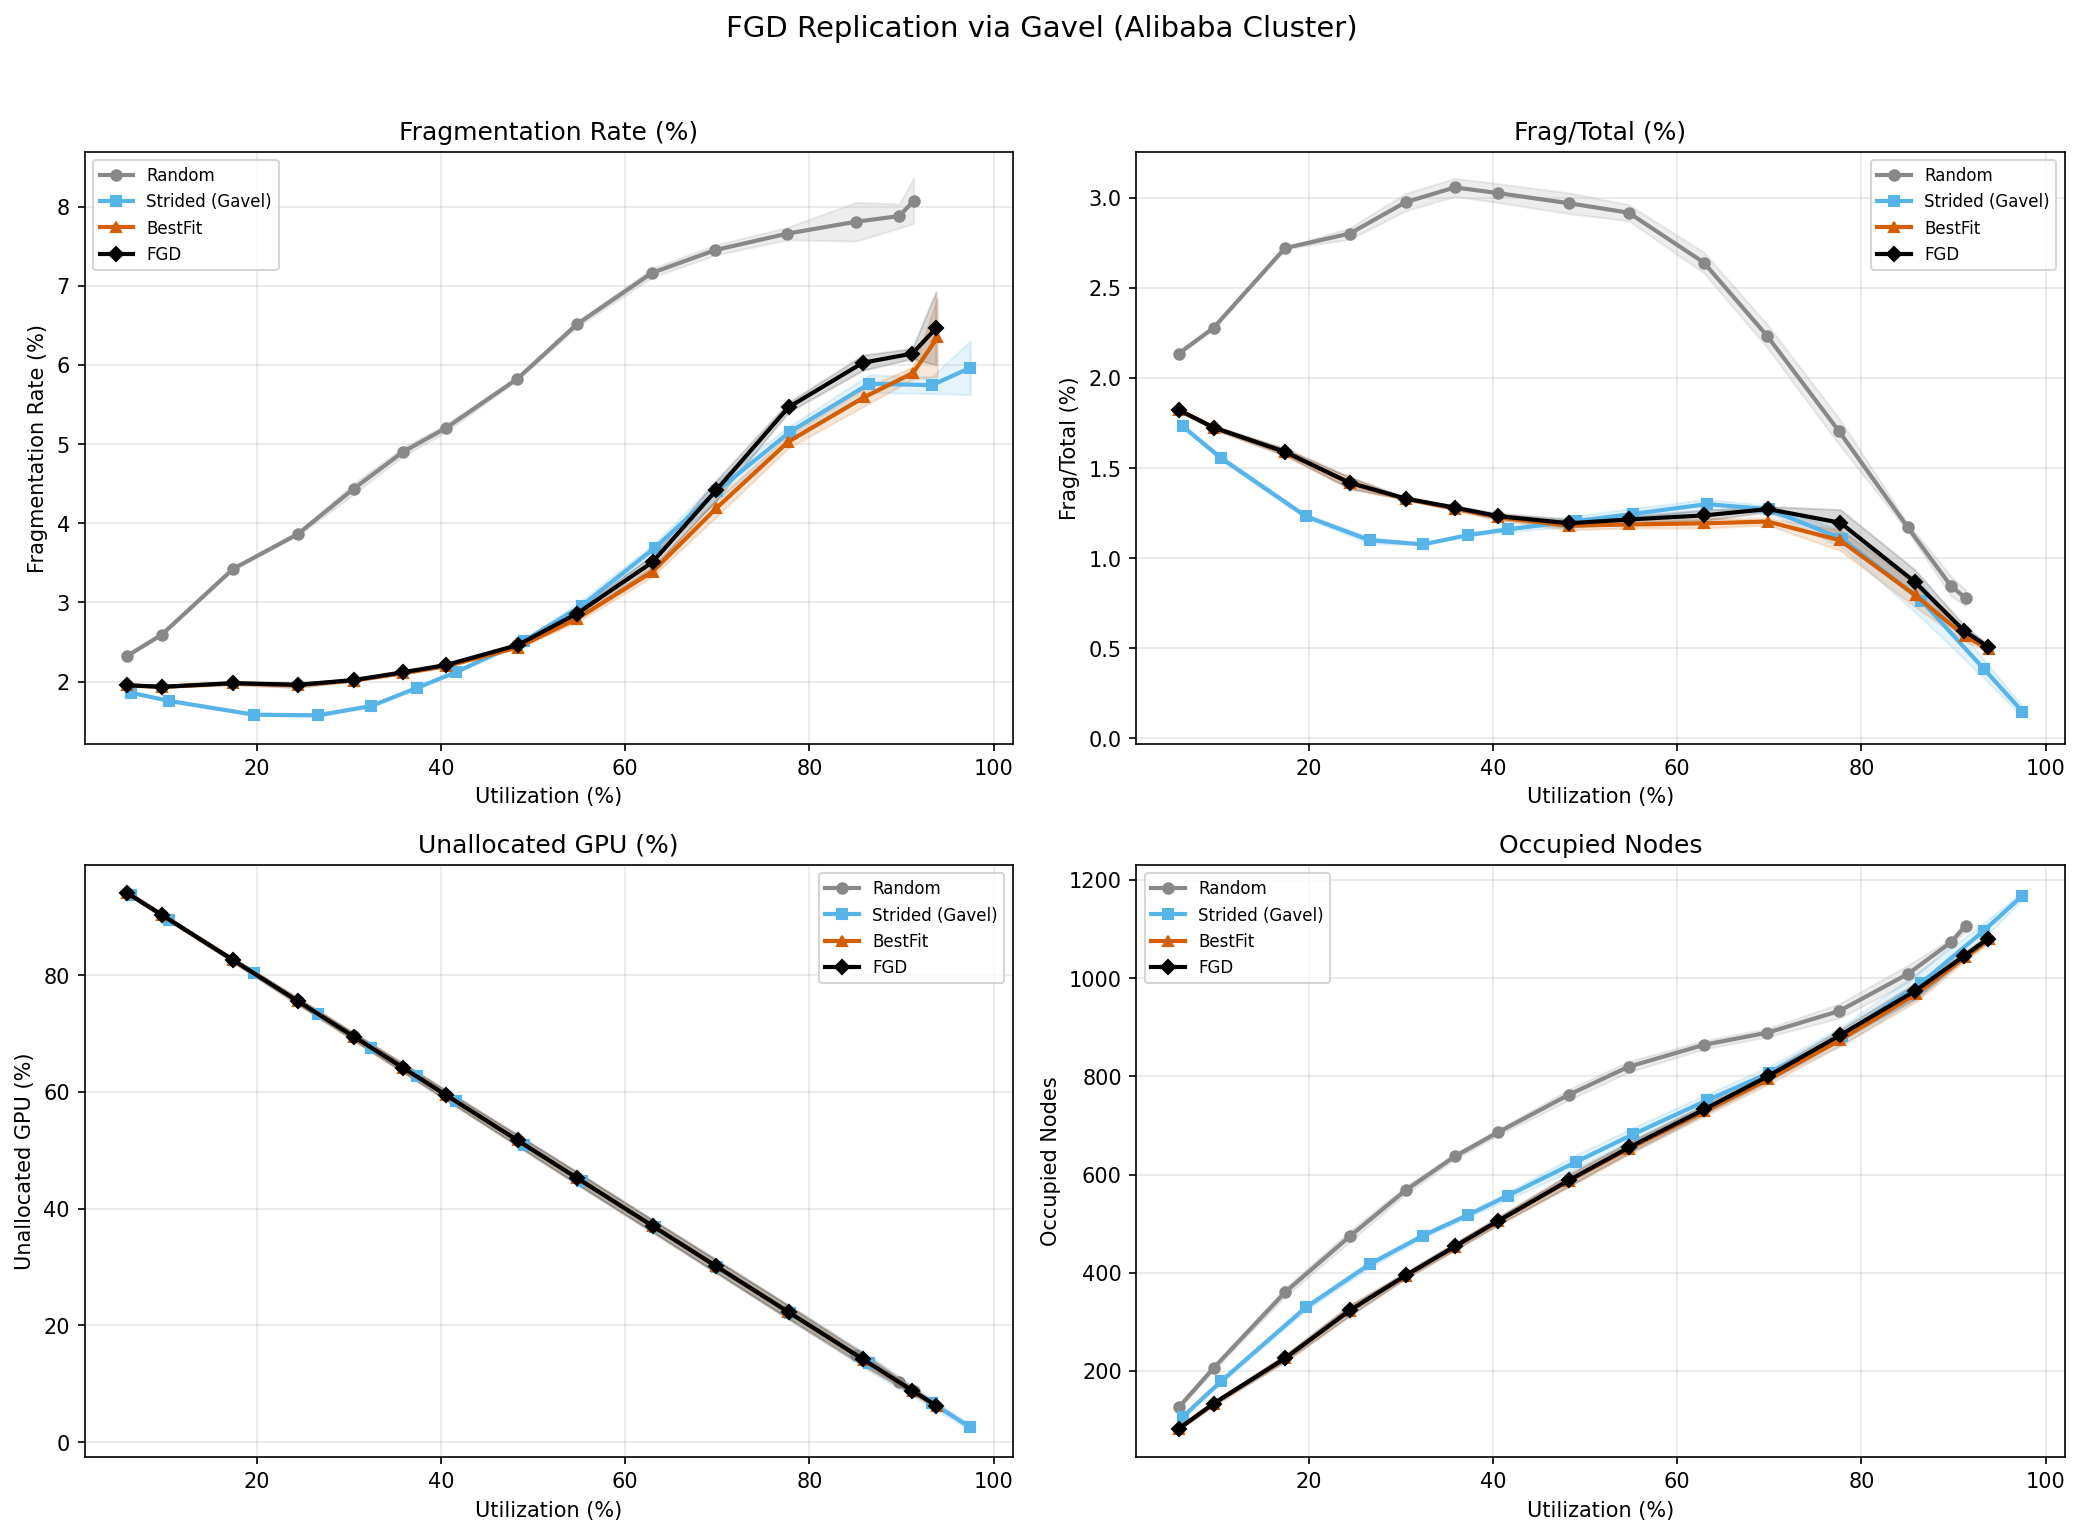
\includegraphics[width=\columnwidth]{fig8_combined_uniform.png}
  \caption{Gavel+FGD on Alibaba Split (uniform 8-GPU nodes). All placement strategies converge -- fragmentation rates are identical regardless of placement policy. Node topology uniformity eliminates the fragmentation problem FGD targets.}
  \label{fig:combined_uniform}
\end{figure}


\section{Analysis}

\subsection{The Role of Node Topology}
The contrast between Fig.~\ref{fig:combined_cluster_h} and Fig.~\ref{fig:combined_uniform} reveals the central finding of our evaluation: \textbf{fragmentation-aware placement matters only when clusters have diverse node sizes.}

Fig.~\ref{fig:topology} illustrates why.
On uniform-node clusters (left), any job that fits on one node fits equally well on any other node of the same type.
The placement decision is trivial because all choices produce the same fragmentation.
On mixed-node clusters (right), a 3-GPU job cannot use scattered 1-GPU fragments across different nodes, so placement decisions directly determine whether capacity remains usable.

This finding has practical implications.
Cloud providers building new clusters with uniform node sizes (e.g., standard 8-GPU servers) gain little from fragmentation-aware placement.
However, clusters that accumulate heterogeneous hardware over time -- mixing older 1--2 GPU machines with newer 4--8 GPU servers -- benefit substantially from FGD-style placement.

\subsection{Policy Independence of Placement Effects}
Our evaluation under both Max-Min Fairness and FIFO allocation policies shows that FGD's placement benefit is consistent regardless of the allocation policy.
On Cluster H, the fragmentation reduction from FGD is 30--40\% under both policies, with nearly identical curves.
This separation of concerns validates our two-stage design: the allocation policy and placement strategy operate on orthogonal dimensions of the scheduling problem.

\subsection{Gavel at Alibaba Scale}
Running Gavel's LP-based allocation on the Alibaba cluster (6,200 GPUs, up to 1,700 concurrent jobs) revealed performance bottlenecks not present at Philly scale (108 GPUs, 50 jobs).
At Alibaba scale, the LP solver consumes 48\% of per-round runtime (3.0s per solve), compared to 8\% at Philly scale.
We addressed this through solver warm-starting and logging optimizations, reducing per-round time from 1.58s to 0.64s -- sufficient for our evaluation but highlighting that Gavel's LP formulation faces scalability limits at production cluster sizes.

\subsection{Improvements}
% Jiayu: distribution shift experiments and additional policy analysis
(Jiayu)

\section{Conclusion}

We presented an integrated GPU cluster scheduler combining Gavel's heterogeneity-aware allocation with FGD's fragmentation-aware placement.
Through replication of both systems (504 Gavel experiments on Philly, standalone FGD on Alibaba) and 900 combined experiments across two cluster topologies, we demonstrated that:

\begin{enumerate}
\item Gavel's heterogeneity-aware policies reduce JCT by 20--70\% compared to heterogeneity-agnostic baselines, and this benefit holds at Alibaba scale.
\item FGD placement reduces fragmentation by 30--40\% on clusters with mixed node sizes (1--8 GPUs per node).
\item Fragmentation-aware placement provides no benefit on uniform-node clusters, where all strategies converge.
\end{enumerate}

The central insight is that fragmentation in GPU clusters is driven by \textit{node topology diversity} -- the variance in GPUs-per-node -- rather than GPU type heterogeneity.
This suggests that cluster architects can mitigate fragmentation either through hardware homogeneity (uniform node sizes) or through software (FGD-style placement).
Our two-stage design demonstrates that these approaches compose cleanly: allocation policy and placement strategy address orthogonal concerns and can be independently selected.

Future work includes extending the evaluation to GPU-sharing workloads with partial allocations (sub-GPU granularity), evaluating migration-aware policies that account for job relocation costs, and profiling the combined system under production-scale job churn.


\newpage
\section*{Acknowledgment}

Thank you to our course instructors, Dr. Keith Winstein and Dr. David Mazi\`eres, for their continued support with and feedback on our project topic, research contribution, and course support.
We recommend all Computer Science students with the ability to take CS244 do so in order to conduct similar projects.


\section*{AI Usage}
To complete this project within the constrained quarter-based timeline, we integrated AI as part of our development work for automating experiment testing scripts, parsing the content of both research works, and code generation for outlining system components -- not end-to-end implementation.
This approach enabled a more comprehensive evaluation and visual aids to support the analysis of our combined Gavel+FGD system.
The ideas and methods are our own; we used AI tools to maximize productivity.


\begin{thebibliography}{00}
\bibitem{GAVEL} Narayanan, D., Santhanam, K., Kazhamiaka, F., et al. ``Heterogeneity-Aware Cluster Scheduling Policies for Deep Learning Workloads.'' OSDI 2020. \href{https://www.usenix.org/conference/osdi20/presentation/narayanan-deepak}{Usenix Web Link}.
\bibitem{FGD} Weng, Q., Yang, L., Yu, Y., et al. ``Beware of Fragmentation: Scheduling GPU-Sharing Workloads with Fragmentation Gradient Descent.'' USENIX ATC 2023. \href{https://www.usenix.org/conference/atc23/presentation/weng}{Usenix Web Link}.
\bibitem{ALIBABA} Alibaba Group. ``Cluster Data Collected from Production Clusters.'' 2020-2023. \href{https://github.com/alibaba/clusterdata}{GitHub Web Link}.
\bibitem{SALUS} Yu, P. and Chowdhury, M. ``Salus: Fine-Grained GPU Sharing Primitives for Deep Learning Applications.'' MLSys, 2020. \href{https://arxiv.org/abs/1902.04610}{arXiv:1902.04610}.
\bibitem{GANDIVA} Xiao, W., Bhardwaj, R., Ramjee, R., et al. ``Gandiva: Introspective Cluster Scheduling for Deep Learning.'' OSDI 2018. \href{https://www.usenix.org/conference/osdi18/presentation/xiao}{Usenix Web Link}.
\bibitem{TIRESIAS} Gu, J., Chowdhury, M., Shin, K.G., et al. ``Tiresias: A GPU Cluster Manager for Distributed Deep Learning.'' NSDI 2019. \href{https://www.usenix.org/conference/nsdi19/presentation/gu}{Usenix Web Link}.
\end{thebibliography}

\appendix
\section{Supplementary Figures}

\begin{figure}[h]
  \centering
  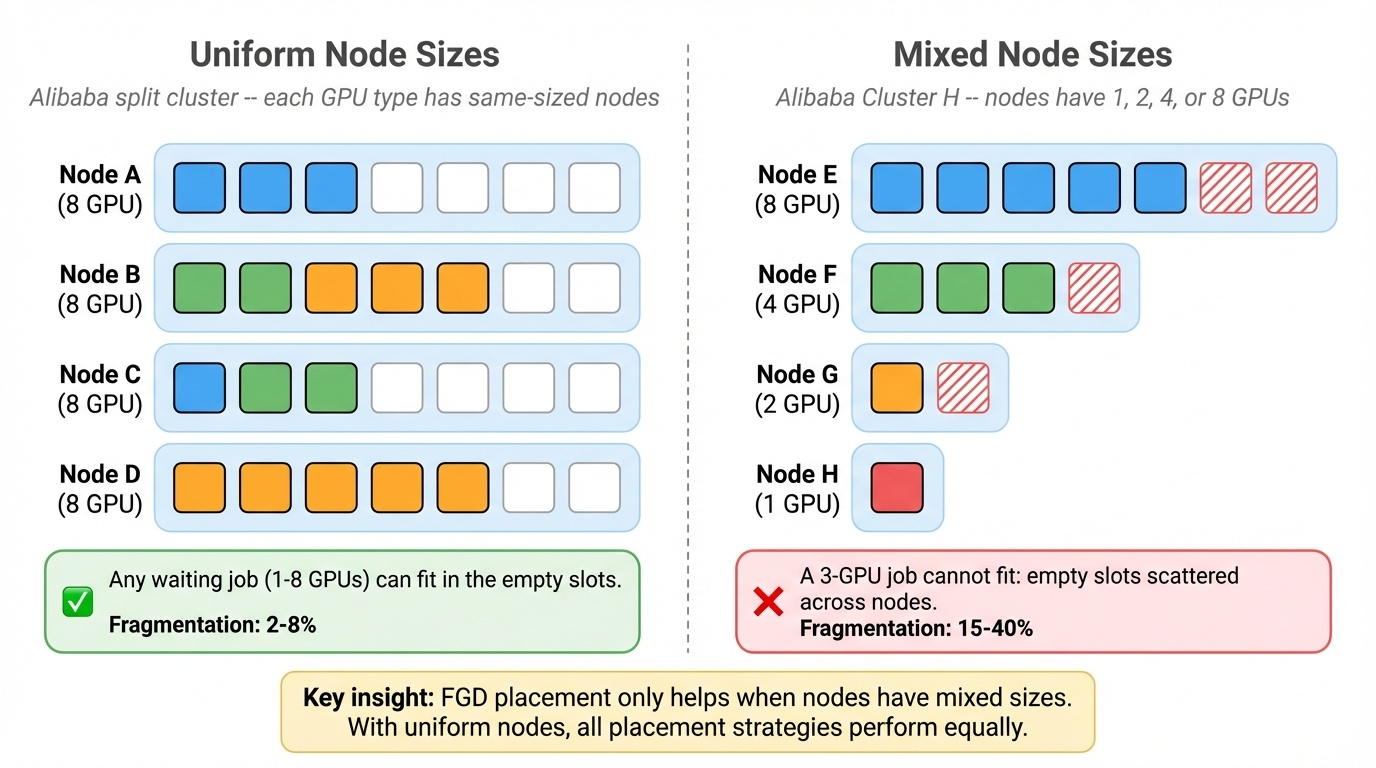
\includegraphics[width=\columnwidth]{fig2_topology.png}
  \caption{Node topology determines fragmentation severity. Left: uniform 8-GPU nodes produce 2--8\% fragmentation regardless of placement. Right: mixed node sizes (1--8 GPUs) produce 15--40\% fragmentation because scattered fragments across small nodes cannot be consolidated. FGD placement helps only in the mixed case.}
  \label{fig:topology}
\end{figure}

\end{document}
